% !TEX spellcheck = en_US



% ~~~~~~~~~~~~~~~~~~~~~~~~~~~~~~~~~~~~~~~ V
% (NC) 2026 Haluk Bingol
% github.com/halukbingol/LaTeX-Templates
%
% Licensees may copy, distribute, display, and perform the work and make derivative works 
% and remixes based on it only for non-commercial purposes. 
% ~~~~~~~~~~~~~~~~~~~~~~~~~~~~~~~~~~~~~~~ A




% =====================================================================
%  Git -- The Concepts
%  ---------------------------------------------------------------------
%  Built on hblib/Template/hblibTemplate.tex with the libraries in ../../hblib/.
%  Programs and their real outputs are in codeoutput/:
%     codeoutput/<Name>.java  a program (classes without main() are only compiled)
%     codeoutput/<Name>.sh    a terminal session, run in a copy of codeoutput/<Name>/
%     codeoutput/<Name>.txt   what it printed, made by:  bash run_examples.sh
% =====================================================================

\documentclass[aspectratio=169,10pt,compress]{beamer}

% ~~~~~~~~~~~~~~~~~~~~~~~~~~~~~~~~~~~~~~~~~~~~~~~~~~~~~~~~~~~~~~~~~ V hblib
	\usepackage{../../hblib/hblibPresentation} % lib presentation: theme, i/N, \hSection, algorithm2e, ...
	\usepackage{../../hblib/hblibCodeoutput} % lib code + output: \lstcode, \lstterminal, ...
	\usepackage{../../hblib/hblibDatastructures} % lib data structures: \hString, \hStack, \hQueue
% ~~~~~~~~~~~~~~~~~~~~~~~~~~~~~~~~~~~~~~~~~~~~~~~~~~~~~~~~~~~~~~~~~ A hblib


% xcolor, array (and the L{width} column), listings, tikz and algorithm2e come from the hblib libraries
\usepackage[T1]{fontenc}
\usepackage{lmodern}
\usepackage{booktabs}

\newcommand{\win}{\textbf{Windows}}
\newcommand{\mac}{\textbf{macOS}}

% algorithm2e set-up (the package is loaded by hblibPresentation)
\SetAlCapFnt{\small}
\SetAlCapNameFnt{\small}
\SetKwProg{Fn}{function}{}{end}
\SetKw{KwError}{error}

% ---------------------------------------------------------------------
\title{Git}
\subtitle{The Concepts}
\author[Bingol]{Haluk O. Bingol}

\institute[FCIS]{
    Faculty of Computer and Information Sciences\\
    Yeditepe University
}
\date{
	{\tiny \hbTimeStamp}
}

\begin{document}




% ~~~~~~~~~~~~~~~~~~~~~~~~~~~~~~~~~~~~~~ V frm
\begin{frame}[t,fragile]
  \titlepage
\end{frame}
% ~~~~~~~~~~~~~~~~~~~~~~~~~~~~~~~~~~~~~~ A frm




% ~~~~~~~~~~~~~~~~~~~~~~~~~~~~~~~~~~~~~~ V frm
\begin{frame}[t,fragile] \frametitle{Outline}
  \begin{columns}[T]
    \begin{column}{0.48\textwidth}
      \tableofcontents[sections={1-5}, hideallsubsections]
    \end{column}
    \begin{column}{0.48\textwidth}
      \tableofcontents[sections={6-10}, hideallsubsections]
    \end{column}
  \end{columns}
\end{frame}
% ~~~~~~~~~~~~~~~~~~~~~~~~~~~~~~~~~~~~~~ A frm

% ~~~~~~~~~~~~~~~~~~~~~~~~~~~~~~~~~~~~~~ V
\hSection[Why]{Why Version Control?}
% ~~~~~~~~~~~~~~~~~~~~~~~~~~~~~~~~~~~~~~ A




% ~~~~~~~~~~~~~~~~~~~~~~~~~~~~~~~~~~~~~~ V frm
\begin{frame}[t,fragile] \frametitle{Life without version control}
  \begin{columns}[T]
    \begin{column}{0.46\textwidth}


% +++++++++++++++++++++++++++++++++++++++ V lst
%: -Lst.
\begin{lstlisting}[style=codesnippet, language={}, basicstyle=\ttfamily\footnotesize]
odev.java
odev_v2.java
odev_v2_final.java
odev_v2_final_REALLY.java
odev_v3_ali_fix.java
\end{lstlisting}
% +++++++++++++++++++++++++++++++++++++++ A lst


    \end{column}
    \begin{column}{0.5\textwidth}
      \begin{itemize}\small
        \item Which one is the newest? What changed between two of them, and why?
        \item Two people edit the same file: whose changes win?
        \item ``It worked yesterday'': what did I change since then?
        \item The laptop dies: where is the backup?
      \end{itemize}
    \end{column}
  \end{columns}
  \begin{block}{A version control system \dots}
    \small records \textbf{every version} of a project, \textbf{who} changed \textbf{what} and \textbf{why}, lets you go back to any version,
    and merges the work of many people.
  \end{block}
\end{frame}
% ~~~~~~~~~~~~~~~~~~~~~~~~~~~~~~~~~~~~~~ A frm




% ~~~~~~~~~~~~~~~~~~~~~~~~~~~~~~~~~~~~~~ V frm
\begin{frame}[t,fragile] \frametitle{Git}
  \begin{itemize}
    \item Written by Linus Torvalds in 2005 for the Linux kernel; today the most used version control system.
    \item \textbf{Distributed}: every copy of a repository has the \textbf{complete history}. You can commit, branch and look at
          history offline; a server (GitHub, GitLab, Bitbucket, your university's) is just another copy.
    \item Fast, and designed for many branches and merges.
    \item Git is the tool; \textbf{GitHub} is a web service that hosts Git repositories and adds pull requests, issues, CI.
  \end{itemize}
  \begin{center}
  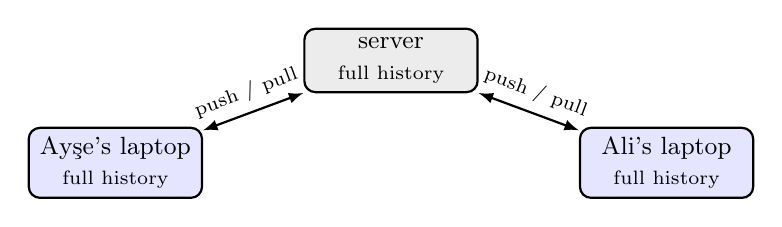
\begin{tikzpicture}[repo/.style={draw, thick, rounded corners, minimum width=2.2cm, minimum height=0.8cm, align=center, font=\small}]
    \node[repo, fill=gray!15] (s) at (0,0) {server\\ \scriptsize full history};
    \node[repo, fill=blue!10] (a) at (-3.5,-1.3) {Ayşe's laptop\\ \scriptsize full history};
    \node[repo, fill=blue!10] (b) at (3.5,-1.3) {Ali's laptop\\ \scriptsize full history};
    \draw[latex-latex, thick] (a) -- node[above, sloped, font=\scriptsize] {push / pull} (s);
    \draw[latex-latex, thick] (b) -- node[above, sloped, font=\scriptsize] {push / pull} (s);
  \end{tikzpicture}
  \end{center}
\end{frame}
% ~~~~~~~~~~~~~~~~~~~~~~~~~~~~~~~~~~~~~~ A frm

% ~~~~~~~~~~~~~~~~~~~~~~~~~~~~~~~~~~~~~~ V
\hSection[Install]{Getting Git}
% ~~~~~~~~~~~~~~~~~~~~~~~~~~~~~~~~~~~~~~ A




% ~~~~~~~~~~~~~~~~~~~~~~~~~~~~~~~~~~~~~~ V frm
\begin{frame}[t,fragile] \frametitle{Installing and configuring Git}
  \begin{columns}[T]
    \begin{column}{0.48\textwidth}
      \begin{block}{Windows (Command Prompt)}


% +++++++++++++++++++++++++++++++++++++++ V lst
%: -Lst.
\begin{lstlisting}[style=codesnippet, language={}, basicstyle=\ttfamily\scriptsize]
winget install --id Git.Git -e
rem or the installer from git-scm.com
rem it includes "Git Bash"
git --version
\end{lstlisting}
% +++++++++++++++++++++++++++++++++++++++ A lst


      \end{block}
    \end{column}
    \begin{column}{0.48\textwidth}
      \begin{block}{macOS (Terminal)}


% +++++++++++++++++++++++++++++++++++++++ V lst
%: -Lst.
\begin{lstlisting}[style=codesnippet, language=bash, basicstyle=\ttfamily\scriptsize]
xcode-select --install
# or: brew install git
git --version
\end{lstlisting}
% +++++++++++++++++++++++++++++++++++++++ A lst


      \end{block}
    \end{column}
  \end{columns}

  \vspace{0.2em}
  \small Once per computer, the same on both systems (your name and e-mail go into every commit):


% +++++++++++++++++++++++++++++++++++++++ V lst
%: -Lst.
\begin{lstlisting}[style=codesnippet, language=bash, basicstyle=\ttfamily\scriptsize]
git config --global user.name "Ayşe Yılmaz"
git config --global user.email "ayse@example.com"
git config --global init.defaultBranch main
\end{lstlisting}
% +++++++++++++++++++++++++++++++++++++++ A lst


  \small \win: also \texttt{git config --global core.autocrlf true} (line endings; the installer usually sets it).
\end{frame}
% ~~~~~~~~~~~~~~~~~~~~~~~~~~~~~~~~~~~~~~ A frm

% ~~~~~~~~~~~~~~~~~~~~~~~~~~~~~~~~~~~~~~ V
\hSection[Commits]{Commits Are Snapshots}
% ~~~~~~~~~~~~~~~~~~~~~~~~~~~~~~~~~~~~~~ A




% ~~~~~~~~~~~~~~~~~~~~~~~~~~~~~~~~~~~~~~ V frm
\begin{frame}[t,fragile] \frametitle{A commit is a snapshot of the whole project}
  \begin{columns}[T]
    \begin{column}{0.5\textwidth}
      \begin{center}
      \begin{tikzpicture}[scale=1.0, transform shape]
  \node[hcommit] (a1) at (0.0,0.0) {a1};
  \node[hcommit] (b2) at (1.15,0.0) {b2};
  \node[hcommit, hhot] (c3) at (2.3,0.0) {c3};
  \draw[hparent] (b2) -- (a1);
  \draw[hparent] (c3) -- (b2);
  \node[hbranch, above=3pt of c3] (L0) {main};
  \node[hheadref, above=3pt of L0] (L1) {HEAD};
\end{tikzpicture}
      \end{center}
      \small Each circle is a commit; the arrow points to its \textbf{parent}, the commit it was made from.
    \end{column}
    \begin{column}{0.46\textwidth}
      A \textbf{commit} stores
      \begin{itemize}\small
        \item a snapshot of \textbf{all} tracked files (unchanged files are shared, not copied)
        \item the author, the date and a \textbf{message}
        \item its parent commit(s)
      \end{itemize}
      It is named by a \textbf{hash} of all this: 40 hex digits such as \texttt{1187bc9\dots}, usually shortened to 7.
    \end{column}
  \end{columns}
\end{frame}
% ~~~~~~~~~~~~~~~~~~~~~~~~~~~~~~~~~~~~~~ A frm




% ~~~~~~~~~~~~~~~~~~~~~~~~~~~~~~~~~~~~~~ V frm
\begin{frame}[t,fragile] \frametitle{Content addressing: names from contents}
  \begin{itemize}
    \item Git computes a SHA-1 hash of every object (file content, folder, commit): the hash \textbf{is} its name.
    \item Same content $\Rightarrow$ same name: identical files are stored once.
    \item Change one byte $\Rightarrow$ a different name, and different names for every commit after it.
          History cannot be changed silently.
    \item A commit hash identifies the \textbf{entire} history up to that commit.
  \end{itemize}
  \[
  	\mathrm{id}(c) = \mathrm{SHA1}(\text{tree} \mid \text{parents} \mid \text{author} \mid \text{date} \mid \text{message})
  \]
  \small New repositories can use SHA-256 instead (\texttt{git init --object-format=sha256}); see the senior deck.
\end{frame}
% ~~~~~~~~~~~~~~~~~~~~~~~~~~~~~~~~~~~~~~ A frm

% ~~~~~~~~~~~~~~~~~~~~~~~~~~~~~~~~~~~~~~ V
\hSection[Areas]{Working Tree, Staging Area, Repository}
% ~~~~~~~~~~~~~~~~~~~~~~~~~~~~~~~~~~~~~~ A




% ~~~~~~~~~~~~~~~~~~~~~~~~~~~~~~~~~~~~~~ V frm
\begin{frame}[t,fragile] \frametitle{Three places for every file}
  \begin{center}
  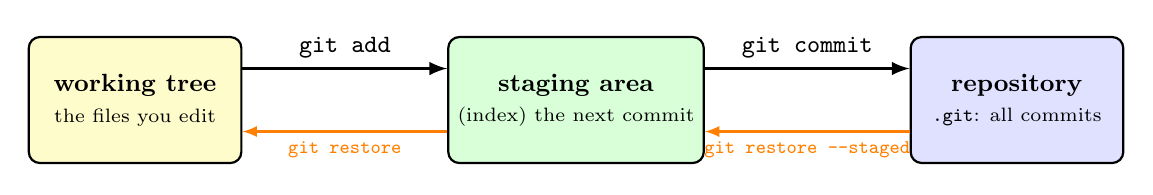
\begin{tikzpicture}[area/.style={draw, thick, rounded corners, minimum width=2.7cm, minimum height=1.6cm, align=center, font=\small}]
    \node[area, fill=yellow!20] (w) at (0,0)    {\textbf{working tree}\\ \scriptsize the files you edit};
    \node[area, fill=green!15]  (i) at (5.6,0)  {\textbf{staging area}\\ \scriptsize (index) the next commit};
    \node[area, fill=blue!12]   (r) at (11.2,0) {\textbf{repository}\\ \scriptsize \texttt{.git}: all commits};
    \draw[-latex, very thick] ([yshift=4mm]w.east) -- node[above, font=\ttfamily\small] {git add} ([yshift=4mm]i.west);
    \draw[-latex, very thick] ([yshift=4mm]i.east) -- node[above, font=\ttfamily\small] {git commit} ([yshift=4mm]r.west);
    \draw[-latex, thick, orange] ([yshift=-4mm]i.west) -- node[below, font=\ttfamily\scriptsize] {git restore} ([yshift=-4mm]w.east);
    \draw[-latex, thick, orange] ([yshift=-4mm]r.west) -- node[below, font=\ttfamily\scriptsize] {git restore -{}-staged} ([yshift=-4mm]i.east);
  \end{tikzpicture}
  \end{center}
  \begin{itemize}\small
    \item You choose \textbf{what} goes into the next commit with \texttt{git add}: one logical change per commit, even if you edited more.
    \item \texttt{git status} tells you, for every changed file, in which of the three places it differs.
    \item \texttt{git diff}: working tree vs staging area; \texttt{git diff -{}-staged}: staging area vs last commit.
  \end{itemize}
\end{frame}
% ~~~~~~~~~~~~~~~~~~~~~~~~~~~~~~~~~~~~~~ A frm




% ~~~~~~~~~~~~~~~~~~~~~~~~~~~~~~~~~~~~~~ V frm
\begin{frame}[t,fragile] \frametitle{The life of a file}
  \begin{center}
  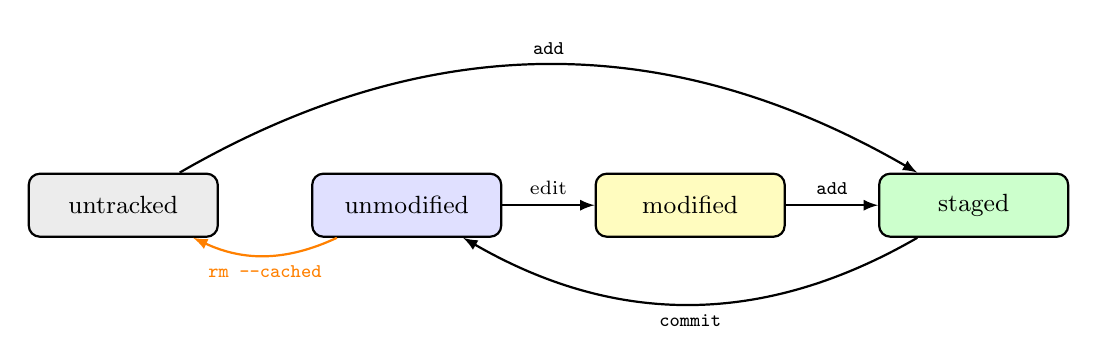
\begin{tikzpicture}[st/.style={draw, thick, rounded corners, minimum width=2.4cm, minimum height=0.8cm, font=\small}]
    \node[st, fill=gray!15]   (u) at (0,0)    {untracked};
    \node[st, fill=blue!12]   (c) at (3.6,0)  {unmodified};
    \node[st, fill=yellow!25] (m) at (7.2,0)  {modified};
    \node[st, fill=green!20]  (s) at (10.8,0) {staged};
    \draw[-latex, thick] (u) to[bend left=30] node[above, font=\ttfamily\scriptsize] {add} (s);
    \draw[-latex, thick] (c) -- node[above, font=\scriptsize] {edit} (m);
    \draw[-latex, thick] (m) -- node[above, font=\ttfamily\scriptsize] {add} (s);
    \draw[-latex, thick] (s) to[bend left=30] node[below, font=\ttfamily\scriptsize] {commit} (c);
    \draw[-latex, thick, orange] (c) to[bend left=25] node[below, font=\ttfamily\scriptsize] {rm -{}-cached} (u);
  \end{tikzpicture}
  \end{center}
  \small A file that Git should never track (build output, \texttt{.class} files, passwords) goes into \texttt{.gitignore}; it stays
  \emph{untracked} and \texttt{git status} stops mentioning it.
\end{frame}
% ~~~~~~~~~~~~~~~~~~~~~~~~~~~~~~~~~~~~~~ A frm




% ~~~~~~~~~~~~~~~~~~~~~~~~~~~~~~~~~~~~~~ V frm
\begin{frame}[t,fragile] \frametitle{What \texttt{git commit} does}
  \begin{columns}[T]
    \begin{column}{0.6\textwidth}
      \SetAlFnt{\small}


% +++++++++++++++++++++++++++++++++++++++ V alg
%: -Alg. 
\begin{algorithm}[H]
  \caption{Commit}
  \KwIn{the staging area $I$, the current branch $b$, a message $m$}
  \lIf{$I$ equals the snapshot of the last commit}{\KwError{nothing to commit}}
  store every file of $I$ as a \textbf{blob} (if not stored yet)\;
  store the folders of $I$ as \textbf{trees} of blob and tree names\;
  $p \gets$ the commit that $b$ points to\;
  $c \gets$ a new \textbf{commit} object (root tree, parent $p$, author, date, $m$)\;
  move $b$ to $c$\;
\end{algorithm}
% +++++++++++++++++++++++++++++++++++++++ A alg

    \end{column}
    \begin{column}{0.36\textwidth}
      \begin{itemize}\small
        \item Nothing is ever overwritten: new objects are \textbf{added}.
        \item The only thing that changes is the branch: a small file with a commit hash.
        \item That is why Git is fast and why lost work can almost always be found again (\texttt{git reflog}).
      \end{itemize}
    \end{column}
  \end{columns}
\end{frame}
% ~~~~~~~~~~~~~~~~~~~~~~~~~~~~~~~~~~~~~~ A frm

% ~~~~~~~~~~~~~~~~~~~~~~~~~~~~~~~~~~~~~~ V
\hSection[Objects]{Inside the Repository}
% ~~~~~~~~~~~~~~~~~~~~~~~~~~~~~~~~~~~~~~ A




% ~~~~~~~~~~~~~~~~~~~~~~~~~~~~~~~~~~~~~~ V frm
\begin{frame}[t,fragile] \frametitle{Four kinds of objects}
  \begin{columns}[T]
    \begin{column}{0.56\textwidth}
      \begin{center}
      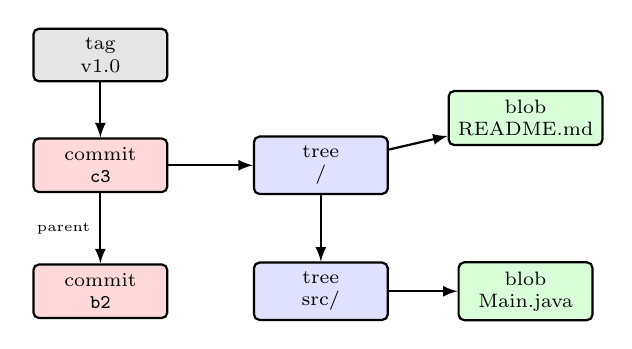
\begin{tikzpicture}[ob/.style={draw, thick, rounded corners=2pt, minimum width=1.7cm, minimum height=0.6cm, font=\scriptsize, align=center}]
        \node[ob, fill=red!15]    (c)  at (0,0)     {commit\\ \texttt{c3}};
        \node[ob, fill=red!15]    (p)  at (0,-1.6)  {commit\\ \texttt{b2}};
        \node[ob, fill=blue!12]   (t)  at (2.8,0)   {tree\\ /};
        \node[ob, fill=blue!12]   (t2) at (2.8,-1.6) {tree\\ src/};
        \node[ob, fill=green!15]  (b1) at (5.4,0.6)  {blob\\ README.md};
        \node[ob, fill=green!15]  (b2) at (5.4,-1.6) {blob\\ Main.java};
        \node[ob, fill=gray!20]   (g)  at (0,1.4)    {tag\\ v1.0};
        \draw[-latex, thick] (c) -- node[left, font=\tiny] {parent} (p);
        \draw[-latex, thick] (c) -- (t);
        \draw[-latex, thick] (t) -- (b1);
        \draw[-latex, thick] (t) -- (t2);
        \draw[-latex, thick] (t2) -- (b2);
        \draw[-latex, thick] (g) -- (c);
      \end{tikzpicture}
      \end{center}
    \end{column}
    \begin{column}{0.42\textwidth}
      \begin{itemize}\small
        \item \textbf{blob}: the content of one file (no name)
        \item \textbf{tree}: a folder: names $\to$ blobs and trees
        \item \textbf{commit}: a root tree, parents, author, message
        \item \textbf{tag}: a named, annotated pointer to a commit (a release)
      \end{itemize}
      \small A commit's history is a \textbf{graph}; its snapshot is a \textbf{tree} of folders. Both are made of the same objects in \texttt{.git/objects}.
    \end{column}
  \end{columns}
\end{frame}
% ~~~~~~~~~~~~~~~~~~~~~~~~~~~~~~~~~~~~~~ A frm

% ~~~~~~~~~~~~~~~~~~~~~~~~~~~~~~~~~~~~~~ V
\hSection[Branches]{Branches and HEAD}
% ~~~~~~~~~~~~~~~~~~~~~~~~~~~~~~~~~~~~~~ A




% ~~~~~~~~~~~~~~~~~~~~~~~~~~~~~~~~~~~~~~ V frm
\begin{frame}[t,fragile] \frametitle{A branch is a movable pointer}
  \begin{columns}[T]
    \begin{column}{0.54\textwidth}
      \begin{center}
      \begin{tikzpicture}[scale=1.0, transform shape]
  \node[hcommit] (a1) at (0.0,0.0) {a1};
  \node[hcommit] (b2) at (1.15,0.0) {b2};
  \node[hcommit, hhot] (c3) at (2.3,0.0) {c3};
  \draw[hparent] (b2) -- (a1);
  \draw[hparent] (c3) -- (b2);
  \node[hbranch, above=3pt of c3] (L0) {main};
  \node[hheadref, above=3pt of L0] (L1) {HEAD};
  \node[hbranch, below=3pt of c3] (L2) {feature};
\end{tikzpicture}\\[0.3em]
      \small after \texttt{git branch feature}
      \end{center}
      \begin{center}
      \begin{tikzpicture}[scale=1.0, transform shape]
  \node[hcommit] (a1) at (0.0,0.0) {a1};
  \node[hcommit] (b2) at (1.15,0.0) {b2};
  \node[hcommit] (c3) at (2.3,0.0) {c3};
  \node[hcommit, hhot] (d4) at (3.4499999999999997,0.0) {d4};
  \draw[hparent] (b2) -- (a1);
  \draw[hparent] (c3) -- (b2);
  \draw[hparent] (d4) -- (c3);
  \node[hbranch, above=3pt of c3] (L0) {main};
  \node[hbranch, below=3pt of d4] (L1) {feature};
  \node[hheadref, below=3pt of L1] (L2) {HEAD};
\end{tikzpicture}\\[0.3em]
      \small after \texttt{git switch feature} and one commit
      \end{center}
    \end{column}
    \begin{column}{0.42\textwidth}
      \begin{itemize}\small
        \item A \textbf{branch} is a name for a commit; it moves forward with every new commit on it.
        \item Creating a branch costs nothing: one small file.
        \item \textbf{HEAD} says which branch you are on: the next commit moves \emph{that} branch.
        \item \texttt{git switch} moves HEAD and updates the working tree to that snapshot.
        \item \emph{Detached HEAD}: HEAD points to a commit, not a branch; new commits there belong to no branch.
      \end{itemize}
    \end{column}
  \end{columns}
\end{frame}
% ~~~~~~~~~~~~~~~~~~~~~~~~~~~~~~~~~~~~~~ A frm

% ~~~~~~~~~~~~~~~~~~~~~~~~~~~~~~~~~~~~~~ V
\hSection[Merge]{Merging and Rebasing}
% ~~~~~~~~~~~~~~~~~~~~~~~~~~~~~~~~~~~~~~ A




% ~~~~~~~~~~~~~~~~~~~~~~~~~~~~~~~~~~~~~~ V frm
\begin{frame}[t,fragile] \frametitle{Two kinds of merge}
  \begin{columns}[T]
    \begin{column}{0.48\textwidth}
      \begin{block}{Fast-forward}
        \centering
        \begin{tikzpicture}[scale=0.9, transform shape]
  \node[hcommit] (a1) at (0.0,0.0) {a1};
  \node[hcommit] (b2) at (1.15,0.0) {b2};
  \node[hcommit, hhot] (c3) at (2.3,0.0) {c3};
  \draw[hparent] (b2) -- (a1);
  \draw[hparent] (c3) -- (b2);
  \node[hbranch, above=3pt of c3] (L0) {main};
  \node[hbranch, below=3pt of c3] (L1) {feature};
\end{tikzpicture}\\
        \small \texttt{main} had no new commits: \texttt{git merge feature} just moves \texttt{main} forward.
      \end{block}
    \end{column}
    \begin{column}{0.48\textwidth}
      \begin{block}{Three-way merge}
        \centering
        \begin{tikzpicture}[scale=0.9, transform shape]
  \node[hcommit] (a1) at (0.0,-0.45) {a1};
  \node[hcommit] (b2) at (1.15,0.0) {b2};
  \node[hcommit] (c3) at (1.15,-0.9) {c3};
  \node[hcommit, hhot] (m4) at (2.3,-0.45) {m4};
  \draw[hparent] (b2) -- (a1);
  \draw[hparent] (c3) -- (a1);
  \draw[hparent] (m4) -- (b2);
  \draw[hparent] (m4) -- (c3);
  \node[hbranch, right=3pt of m4] (L0) {main};
  \node[hbranch, below=3pt of c3] (L1) {feature};
\end{tikzpicture}\\
        \small Both branches moved on: Git combines them in a \textbf{merge commit} with \textbf{two parents}.
      \end{block}
    \end{column}
  \end{columns}
\end{frame}
% ~~~~~~~~~~~~~~~~~~~~~~~~~~~~~~~~~~~~~~ A frm




% ~~~~~~~~~~~~~~~~~~~~~~~~~~~~~~~~~~~~~~ V frm
\begin{frame}[t,fragile] \frametitle{How Git merges a file}
  \begin{columns}[T]
    \begin{column}{0.58\textwidth}
      \SetAlFnt{\small}


% +++++++++++++++++++++++++++++++++++++++ V alg
%: -Alg. 
\begin{algorithm}[H]
  \caption{Three-way merge of one file}
  \KwIn{the file in the common ancestor $B$, in ours $O$, in theirs $T$}
  \ForEach{region of the file}{
    \uIf{$O = B$}{take $T$\tcp*{only they changed it}}
    \uElseIf{$T = B$}{take $O$\tcp*{only we changed it}}
    \uElseIf{$O = T$}{take $O$\tcp*{both made the same change}}
    \Else{mark a \textbf{conflict}: keep $O$ and $T$ between markers\;}
  }
\end{algorithm}
% +++++++++++++++++++++++++++++++++++++++ A alg

    \end{column}
    \begin{column}{0.38\textwidth}
      \begin{itemize}\small
        \item The \textbf{merge base} $B$ is the last common ancestor of the two branches.
        \item Most merges need no help.
        \item A \textbf{conflict} happens only when both sides changed the \emph{same lines} differently. You edit the file, \texttt{git add}, \texttt{git commit}.
      \end{itemize}
    \end{column}
  \end{columns}
\end{frame}
% ~~~~~~~~~~~~~~~~~~~~~~~~~~~~~~~~~~~~~~ A frm




% ~~~~~~~~~~~~~~~~~~~~~~~~~~~~~~~~~~~~~~ V frm
\begin{frame}[t,fragile] \frametitle{Rebase: replay commits on a new base}
  \begin{columns}[T]
    \begin{column}{0.5\textwidth}
      \centering
      \begin{tikzpicture}[scale=0.85, transform shape]
  \node[hcommit] (a1) at (0.0,0.0) {a1};
  \node[hcommit] (b2) at (1.15,0.0) {b2};
  \node[hcommit] (c3) at (2.3,0.0) {c3};
  \node[hcommit, hdone] (x4) at (1.15,-0.9) {x4};
  \node[hcommit, hdone] (y5) at (2.3,-0.9) {y5};
  \draw[hparent] (b2) -- (a1);
  \draw[hparent] (c3) -- (b2);
  \draw[hparent] (x4) -- (a1);
  \draw[hparent] (y5) -- (x4);
  \node[hbranch, above=3pt of c3] (L0) {main};
  \node[hbranch, right=3pt of y5] (L1) {feature};
\end{tikzpicture}\\
      \small before \texttt{git rebase main}\\[0.4em]
      \begin{tikzpicture}[scale=0.85, transform shape]
  \node[hcommit] (a1) at (0.0,0.0) {a1};
  \node[hcommit] (b2) at (1.15,0.0) {b2};
  \node[hcommit] (c3) at (2.3,0.0) {c3};
  \node[hcommit, hhot] (x6) at (3.4499999999999997,0.0) {x6};
  \node[hcommit, hhot] (y7) at (4.6,0.0) {y7};
  \draw[hparent] (b2) -- (a1);
  \draw[hparent] (c3) -- (b2);
  \draw[hparent] (x6) -- (c3);
  \draw[hparent] (y7) -- (x6);
  \node[hbranch, above=3pt of c3] (L0) {main};
  \node[hbranch, above=3pt of y7] (L1) {feature};
\end{tikzpicture}\\
      \small after: new commits \texttt{x6}, \texttt{y7}
    \end{column}
    \begin{column}{0.46\textwidth}
      \begin{itemize}\small
        \item Rebase \textbf{copies} each commit of \texttt{feature} on top of \texttt{main}: same changes, new parents, \textbf{new hashes}.
        \item Result: a straight history, no merge commit.
        \item The golden rule: \hRemark{never rebase commits that others already have} (that you pushed to a shared branch).
        \item Merge keeps the true history; rebase makes it tidy. Teams pick one style.
      \end{itemize}
    \end{column}
  \end{columns}
\end{frame}
% ~~~~~~~~~~~~~~~~~~~~~~~~~~~~~~~~~~~~~~ A frm

% ~~~~~~~~~~~~~~~~~~~~~~~~~~~~~~~~~~~~~~ V
\hSection[Remotes]{Remotes}
% ~~~~~~~~~~~~~~~~~~~~~~~~~~~~~~~~~~~~~~ A




% ~~~~~~~~~~~~~~~~~~~~~~~~~~~~~~~~~~~~~~ V frm
\begin{frame}[t,fragile] \frametitle{Your repository and the remote one}
  \begin{columns}[T]
    \begin{column}{0.5\textwidth}
      \begin{center}
      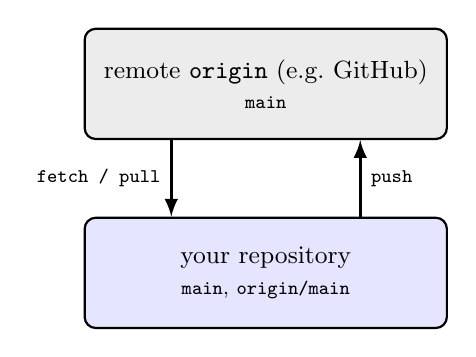
\begin{tikzpicture}[repo/.style={draw, thick, rounded corners, minimum width=4.6cm, minimum height=1.4cm, align=center, font=\small}]
        \node[repo, fill=gray!15] (r) at (0,1.8) {remote \texttt{origin} (e.g.\ GitHub)\\ \scriptsize \texttt{main}};
        \node[repo, fill=blue!10] (l) at (0,-0.6) {your repository\\ \scriptsize \texttt{main}, \texttt{origin/main}};
        \draw[-latex, very thick] ([xshift=-12mm]r.south) -- node[left, font=\ttfamily\scriptsize] {fetch / pull} ([xshift=-12mm]l.north);
        \draw[-latex, very thick] ([xshift=12mm]l.north) -- node[right, font=\ttfamily\scriptsize] {push} ([xshift=12mm]r.south);
      \end{tikzpicture}
      \end{center}
    \end{column}
    \begin{column}{0.46\textwidth}
      \begin{itemize}\small
        \item \texttt{git clone URL}: copy a repository with all its history; the source is called \texttt{origin}.
        \item \texttt{origin/main}: your copy of where \texttt{main} was on the remote when you last talked to it (a \emph{remote-tracking branch}).
        \item \texttt{git fetch}: download new commits, update \texttt{origin/main}; your files do not change.
        \item \texttt{git pull}: fetch, then merge (or rebase) into your branch.
        \item \texttt{git push}: send your commits; refused if the remote has commits you do not have yet.
      \end{itemize}
    \end{column}
  \end{columns}
\end{frame}
% ~~~~~~~~~~~~~~~~~~~~~~~~~~~~~~~~~~~~~~ A frm

% ~~~~~~~~~~~~~~~~~~~~~~~~~~~~~~~~~~~~~~ V
\hSection[Team]{Working Together}
% ~~~~~~~~~~~~~~~~~~~~~~~~~~~~~~~~~~~~~~ A




% ~~~~~~~~~~~~~~~~~~~~~~~~~~~~~~~~~~~~~~ V frm
\begin{frame}[t,fragile] \frametitle{A typical team workflow}
  \begin{columns}[T]
    \begin{column}{0.5\textwidth}
      \begin{enumerate}\small
        \item \texttt{git pull}: start from the latest \texttt{main}
        \item \texttt{git switch -c fix-login}: a branch per task
        \item edit, \texttt{git add}, \texttt{git commit}: small commits
        \item \texttt{git push -u origin fix-login}
        \item open a \textbf{pull request} on GitHub: others review, CI runs the tests
        \item merge into \texttt{main}; delete the branch
      \end{enumerate}
    \end{column}
    \begin{column}{0.46\textwidth}
      \begin{block}{Good commits}
        \small
        \begin{itemize}
          \item one logical change, builds and passes tests
          \item a short summary line ($\le$ 50 characters), imperative: ``Fix null check in login''
          \item a blank line, then \emph{why}, if not obvious
        \end{itemize}
      \end{block}
      \begin{block}{Never commit}
        \small passwords and keys, build output, IDE settings, huge binary files: list them in \texttt{.gitignore}.
      \end{block}
    \end{column}
  \end{columns}
\end{frame}
% ~~~~~~~~~~~~~~~~~~~~~~~~~~~~~~~~~~~~~~ A frm




% ~~~~~~~~~~~~~~~~~~~~~~~~~~~~~~~~~~~~~~ V frm
\begin{frame}[t,fragile] \frametitle{A first taste}
  \lstterminal[basicstyle=\ttfamily\tiny]{codeoutput/Taste.txt}

  \vspace{0.1em}
  \small
  Two commits on \texttt{main}, one on \texttt{idea}, then a merge commit with two parents. \texttt{-{}-graph} draws the history; the
  hashes are real. Same commands on \win{} (Git Bash or Command Prompt) and \mac.
\end{frame}
% ~~~~~~~~~~~~~~~~~~~~~~~~~~~~~~~~~~~~~~ A frm

% ~~~~~~~~~~~~~~~~~~~~~~~~~~~~~~~~~~~~~~ V
\hSection[Summary]{Summary}
% ~~~~~~~~~~~~~~~~~~~~~~~~~~~~~~~~~~~~~~ A




% ~~~~~~~~~~~~~~~~~~~~~~~~~~~~~~~~~~~~~~ V frm
\begin{frame}[t,fragile] \frametitle{Big ideas}
  \begin{itemize}
    \item Git records \textbf{snapshots} (commits) linked to their parents: the history is a graph.
    \item Everything is named by a hash of its content: history cannot change silently.
    \item Three places: working tree $\xrightarrow{\text{add}}$ staging area $\xrightarrow{\text{commit}}$ repository.
    \item A branch is a movable pointer to a commit; HEAD says which branch you are on.
    \item Merge joins histories (fast-forward or merge commit); rebase rewrites them (new hashes).
    \item Every clone is complete; \texttt{fetch}, \texttt{pull} and \texttt{push} synchronise with remotes.
  \end{itemize}
\end{frame}
% ~~~~~~~~~~~~~~~~~~~~~~~~~~~~~~~~~~~~~~ A frm




% ~~~~~~~~~~~~~~~~~~~~~~~~~~~~~~~~~~~~~~ V frm
\begin{frame}[t,fragile] \frametitle{Check yourself}
  \begin{enumerate}\small
    \item What is the difference between Git and GitHub?
    \item You edited three files but want to commit only one. Which command decides that?
    \item Why does changing an old commit change the hashes of all later commits?
    \item Draw the graph after: commit on \texttt{main}, branch \texttt{x}, commit on \texttt{x}, commit on \texttt{main}, merge \texttt{x} into \texttt{main}.
    \item When is a merge a fast-forward? When does it need a merge commit?
    \item Why should you not rebase commits you have already pushed?
  \end{enumerate}
\end{frame}
% ~~~~~~~~~~~~~~~~~~~~~~~~~~~~~~~~~~~~~~ A frm




% ~~~~~~~~~~~~~~~~~~~~~~~~~~~~~~~~~~~~~~ V frm
\begin{frame}[t,fragile]
	\begin{center}
		\vspace{4cm}
		\hRemark{\Huge Questions?}
	\end{center}
\end{frame}
% ~~~~~~~~~~~~~~~~~~~~~~~~~~~~~~~~~~~~~~ A frm



\end{document}
